\clearpage
\section*{Answer Key}
\addcontentsline{toc}{section}{Answer Key}
\label{sec:sample-key}

Every composition scenario in this key was verified by composing the actual
layers with OpenUSD and inspecting the result --- not by reasoning alone.

\Question{1 --- A}
\texttt{defaultPrim}\index{defaultPrim} is layer metadata naming the prim that
consumers compose when they reference or payload the layer \emph{without}
specifying a prim path. It has nothing to do with materials, timeCodes, or
schema definitions.

\Question{2 --- C: (0, 1, 0)}
LIVRPS\index{LIVRPS}: the \emph{Local} opinion in \texttt{scene.usda} is
stronger than anything brought in by the two \emph{References}, so $(0,1,0)$
wins. Between the references themselves, the earlier list entry
(\texttt{chair\_base.usda}) would beat the later one --- relevant only for
opinions the stronger layers do not author.
Figure~\ref{fig:key-q2} makes it visible: a proxy sphere parented under
\texttt{/World/Chair} picks up the composed transform, while gray markers sit
at the four candidate positions.

\begin{figure}[ht]
  \centering
  \begin{tikzpicture}
    \node[anchor=south west, inner sep=0] (img)
      {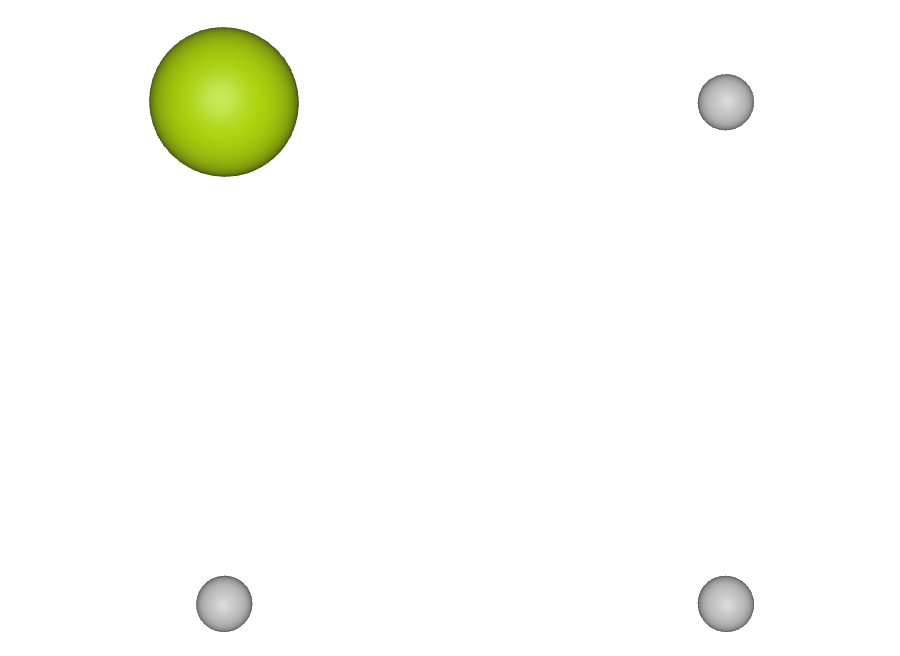
\includegraphics[width=0.62\linewidth]{figures/q02_chair_options.png}};
    \begin{scope}[x={(img.south east)}, y={(img.north west)}]
      \node[notetext] at (0.245,0.185) {A $(0,0,0)$};
      \node[notetext] at (0.80,0.185)  {B $(1,0,0)$};
      \node[notetext] at (0.80,0.72)   {D $(1,1,0)$};
      \node[notetext, draw=usdgreen!60!black, fill=white, rounded corners=1pt]
        (c) at (0.47,0.60) {C $(0,1,0)$ --- composed result};
      \draw[subArc] (c.north west) -- (0.295,0.78);
    \end{scope}
  \end{tikzpicture}
  \caption{Question 2, rendered with \texttt{usdrecord}: gray markers sit at
  the four answer options; the sphere under \texttt{/World/Chair} composes to
  C.}
  \label{fig:key-q2}
\end{figure}

\Question{3 --- A, B, D}
Topology lives in three attributes: \texttt{points},
\texttt{faceVertexCounts}, and \texttt{faceVertexIndices} --- counts say how
many vertices each face consumes, indices say which ones. \texttt{normals}
can be computed (or come from subdivision), and
\texttt{primvars:\allowbreak displayColor} is cosmetic --- both optional.

\Question{4 --- C: 1,500}
Each of the 500 triangular faces consumes three indices:
$500 \times 3 = 1{,}500$ entries. \texttt{faceVertexCounts} would hold 500
entries, each equal to 3.

\Question{5 --- A, B}
Move points $\Rightarrow$ recompute \texttt{extent}\index{extent} (bounds are
authored, not derived on the fly). Change topology $\Rightarrow$ keep
\texttt{faceVertexCounts} consistent with \texttt{faceVertexIndices}. The
pairs in C and D are independent properties, not synchronization invariants.

\Question{6 --- C}
Adding properties to \emph{existing} prim types is what applied API
schemas\index{API schema} do, and those derive from
\texttt{UsdAPISchemaBase}. \texttt{UsdTyped} is the base for IsA (typed)
schemas that define new prim types; \texttt{UsdSchemaBase} is the common
ancestor you do not subclass directly; \texttt{UsdPhysicsBase} does not exist.

\Question{7 --- B, C}
Composition's headline wins are collaboration (people own separate layers of
the same stage without write conflicts) and nondestructive overrides (stronger
opinions on top, original data intact). A confuses USD with version control
--- any file format can live in git. D inverts reality: more layers add
composition cost; they do not optimize access.

\Question{8 --- A, B}
Naming/structure conventions and validation at boundaries are what keep a
pipeline alive as it grows. C is the trap answer: asset structures evolve, so
design for change rather than pretending to finalize one up front. D is dogma
--- production pipelines exchange with DCC-native formats all the time.

\Question{9 --- B}
The \texttt{UsdGeomImageable}\index{UsdGeomImageable} schema carries what
every \emph{renderable} prim needs: \texttt{visibility}, \texttt{purpose},
and primvar plumbing. Concrete geometric properties live further down the
hierarchy (\texttt{Boundable}, \texttt{Gprim}); material assignment belongs to
\texttt{UsdShade} (\texttt{MaterialBindingAPI}).

\Question{10 --- B}
Expose the parameters you expect to vary as inputs on the material's public
interface; consumers then override them per use, instead of forking a material
per combination (C) or hardcoding values (A).

\Question{11 --- B}
\texttt{metersPerUnit}\index{metersPerUnit} is descriptive metadata; USD
performs \emph{no} automatic unit conversion when referencing. Meter-unit
geometry (1.0) interpreted inside a centimeter-unit stage (0.01) reads
100$\times$ too small. Correcting it is the referencing pipeline's job ---
typically a corrective scale on the referencing prim.

\Question{12 --- C}
The export parses cleanly --- verified --- but \texttt{defaultPrim} is
\texttt{World}, and the binding targets \texttt{/Materials/metal}, which lives
\emph{outside} that hierarchy. Reference this layer into another stage and
\texttt{/Materials} never composes; the binding dangles.
\texttt{bindMaterialAs} metadata (A) is legal on a binding relationship;
geom subsets (B) are optional, not required; D inverts the binding model.

\Question{13 --- B}
Composed and verified: the stage \emph{does} resolve
\texttt{loftedColor = blue}, yet the cube stays red. The artist's local
\texttt{over} on \texttt{Cube} in \texttt{main.usda} authors a direct
\texttt{color = red} selection, and a Local opinion beats the selection
authored inside the \texttt{loftedColor} variant (V in LIVRPS). A is backwards
--- the selection in \texttt{contents.usda} is the \emph{weakest} of the
three. C misreads the mechanism: the blue variant does select
\texttt{color = blue}; it simply loses. D is false --- variant selections can
be authored on any prim spec, including in \texttt{main.usda}.
Figure~\ref{fig:key-q13} is the composed stage, rendered.

\begin{figure}[ht]
  \centering
  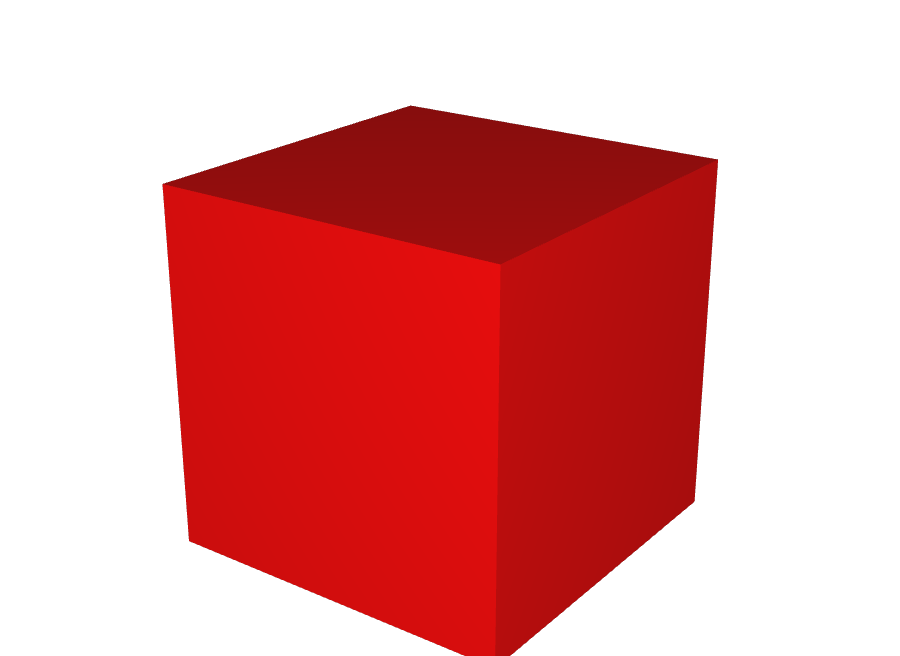
\includegraphics[width=0.42\linewidth]{figures/q13_cube_red.png}
  \caption{Question 13 rendered with \texttt{usdrecord}: the composed stage
  draws a red cube, exactly as answer B predicts.}
  \label{fig:key-q13}
\end{figure}
